

\def\slidemode{%
  \documentclass[fleqn,aspectratio=169]{beamer}
\usepackage{pgfpages}
}
\def\handoutmode{%
  \documentclass[handout,fleqn,aspectratio=169]{beamer}
\usepackage{pgfpages}
\pgfpagesuselayout{resize to}[a4paper,landscape,border shrink=5mm]
}


%\def\pdfmode{handoutmode}
\def\pdfmode{slidemode}

\csname\pdfmode\endcsname

\mode<presentation>
{
  \usetheme{default}
  \usecolortheme{default}
  \usefonttheme{default}
  \setbeamertemplate{navigation symbols}{}
  \setbeamertemplate{caption}[numbered]
  \setbeamertemplate{footline}[frame number]  % or "page number"
  \setbeamercolor{frametitle}{fg=white}
  \setbeamercolor{footline}{fg=black}
} 


\mode<presentation>
{
  \usetheme{default}
  \usecolortheme{default}
  \usefonttheme{default}
  \setbeamertemplate{navigation symbols}{}
  \setbeamertemplate{caption}[numbered]
  \setbeamertemplate{footline}[frame number]  % or "page number"
  \setbeamercolor{frametitle}{fg=white}
  \setbeamercolor{footline}{fg=black}
} 


\usepackage[english]{babel}
%\usepackage[utf8x]{inputenc}
\usepackage{tikz}
\usepackage{courier}
\usepackage{array}
\usepackage{bold-extra}
%\usepackage{minted}
%\usepackage[thicklines]{cancel}
%\usepackage{fancyvrb}
\usepackage{kotex}
\usepackage{paralist}
\usepackage{collectbox}
\usepackage{amsmath}
\usepackage{mathtools}
\usepackage{nccmath}
\usepackage{bm}

\xdefinecolor{dianablue}{rgb}{0.18,0.24,0.31}
\xdefinecolor{darkblue}{rgb}{0.1,0.1,0.7}
\xdefinecolor{darkgreen}{rgb}{0,0.5,0}
\xdefinecolor{darkgrey}{rgb}{0.35,0.35,0.35}
\xdefinecolor{darkorange}{rgb}{0.8,0.5,0}
\xdefinecolor{darkred}{rgb}{0.7,0,0}
\definecolor{darkgreen}{rgb}{0,0.6,0}
\definecolor{mauve}{rgb}{0.58,0,0.82}



\title[]{Lecture 8: Random Processes, Part II}
\author{Yi, Yung (이융)}
\institute{EE210: Probability and Introductory Random Processes\\ KAIST EE}
\date{\today}

\input{../mymath}


\begin{document}

%itemshape
\setbeamertemplate{itemize item}{\scriptsize\raise1.25pt\hbox{\donotcoloroutermaths$\bullet$}}
\setbeamertemplate{itemize subitem}{\tiny\raise1.5pt\hbox{\donotcoloroutermaths$\circ$}}
\setbeamertemplate{itemize subsubitem}{\tiny\raise1.5pt\hbox{\donotcoloroutermaths$\blacktriangleright$}}
%default value for spacing
\plitemsep 0.1in
\pltopsep 0.03in
\setlength{\parskip}{0.15in}
%\setlength{\parindent}{-0.5in}
\setlength{\abovedisplayskip}{0.07in}
\setlength{\mathindent}{0cm}
\setbeamertemplate{frametitle continuation}{[\insertcontinuationcount]}

\setlength{\leftmargini}{0.5cm}
\setlength{\leftmarginii}{0.5cm}

\setlength{\fboxrule}{0.05pt}
\setlength{\fboxsep}{5pt}


\begin{frame}
  \titlepage
\end{frame}

% % Uncomment these lines for an automatically generated outline.
% \begin{frame}{Outline}
% % \tableofcontents
% \plitemsep 0.1in
% \bci
% \item 

% \item 
% \eci
% \end{frame}

% START START START START START START START START START START START START START

%%%%%%%%%%%%%%%%%%%%%%%%%%%%%%%%%%%%%%%%%%%%%%%%%%%%%%
\begin{frame}{Roadmap}

{\Large Markov Chain}


  \plitemsep 0.1in

\bce[(1)]


%\item \redf{Markov Chain}

\item Definition, Transition Probability Matrix, State Transition Diagram

\item $n$-step Transition Probability

\item Classification of States

\item Steady-state Behaviors and Stationary Distribution

\item Transient Behaviors



\ece 

\end{frame}

%%%%%%%%%%%%%%%%%%%%%%%%%%%%%%%%%%%%%%%%%%%%%%%%%%%%%%
\section{L8(1)}
\begin{frame}{Roadmap}

{\Large Markov Chain}


  \plitemsep 0.1in

\bce[(1)]


%\item \redf{Markov Chain}

\item \redf{Definition, Transition Probability Matrix, State Transition Diagram}

\item \grayf{$n$-step Transition Probability

\item Classification of States

\item Steady-state Behaviors and Stationary Distribution

\item Transient Behaviors}



\ece 

\end{frame}

%%%%%%%%%%%%%%%%%%%%%%%%%%%%%%%%%%%%%%%%%%%%%%%%%%%%%%
\begin{frame}{Recap and Markov Chain}

- Assume discrete times $n=1, 2, \ldots$
\vspace{-0.3cm}

\plitemsep 0.05in
\bci 
\item Random process: A sequence of $X_1, X_2, X_3, \cdots $

\item<2-> ``Simplest'' random process

\bci
\item<3-> Process without memory
\aleq{
\cprob{X_{n} = i_{n} \mid X_{n-1} = i_{n-1},X_{n-2} = i_{n-2},X_{n-3} = i_{n-3}, \ldots, X_1 = i_1 } = \magenf{\cprob{X_{n} = i_{n}}}
}
\item<4-> \redf{Bernoulli process}
\eci

\item<5-> A random process that is \orangef{just a little more} general  than the above?
\bci
\item<6-> Process that depends only on ``yesterday", not the entire history
\aleq{
\cprob{X_{n} = i_{n} \mid X_{n-1} = i_{n-1},X_{n-2} = i_{n-2},X_{n-3} = i_{n-3}, \ldots, X_1 = i_1 } = \magenf{\cprob{X_{n} = i_{n} \mid X_{n-1} = i_{n-1} }}
}

\item<7-> \redf{Markov chain}

\item<7-> One of the most popular random processes in engineering!
\eci

\eci 
\end{frame}

%%%%%%%%%%%%%%%%%%%%%%%%%%%%%%%%%%%%%%%%%%%%%%%%%%%%%%
\begin{frame}{Example: Machine Failure, Repair, and Replacement}

\plitemsep 0.1in
\bci 
\item A machine: working or broken down on a given day. 
\bci
\item If working, break down in the next day w.p. $b$, and continue working w.p. $1-b.$

\item If broken down, it will be repaired and be working in the next day w.p. $r,$ and continue to be broken down w.p. $1-r.$ 
\eci

\item<2-> $X_n \in \{1,2 \}$: status of the machine, 1: working and 2: broken down

\item<3-> $(X_n)_{n=1}^\infty$: A random process satisfying: for any $n \ge 1,$
\aleq{
\cprob{X_{n+1} = 1 | X_{n} = 1} = 1-b, \quad \cprob{X_{n+1} = 2 | X_{n} = 1} = b \cr
\cprob{X_{n+1} = 1 | X_{n} = 2} = r,  \quad \cprob{X_{n+1}  = 2 | X_{n} = 2} = 1-r 
}

\item<4-> What will happen at $(n+1)$-th day depends only on what happens at $n$-th day? 
\eci 
\end{frame}


%%%%%%%%%%%%%%%%%%%%%%%%%%%%%%%%%%%%%%%%%%%%%%%%%%%%%%
\begin{frame}{Markov Chain: Definition (1)}

\footnotetext{A Markov chain can be also defined for the infinte
  $\set{S}=\{1, 2, \ldots \},$ but we just focus on the finite state
  space in this lecture.}


  \plitemsep 0.1in

\bci 
\item<2-> \defi Let $X_1, \ldots, X_n, \ldots$ be a sequence of random
  variables taking values in some finite space
  $\set{S}=\{1, 2, \ldots, m\}$, such that   for all $i,j \in
  \set{S},$ $n\geq 0,$ the following \blueblank{3}{Markov property} is
  satisfied:\\
  for all $n \geq 0,$ all $i,j \in \set{S},$ and all possible
  sequences $i_0, \ldots, i_{n-1}$ of earlier states, 
\mycolorbox{
\centering
  \redblank{3}{$\cprob{X_{n+1} = j \vert X_{n} = i}$}  =
  $\cprob{X_{n+1} = j
      \vert X_n = i, X_{n-1}=i_{n-1}, \ldots, X_0=i_0}$
}

\item<4->  \magenf{Alternate definition via conditional independence.}
  For any fixed $n,$ the future of the process after $n$ is {\red independent}
  of $\{X_1, \ldots, X_{n-1} \},$ {\red given} $X_n.$
  % (i.e., depends only on $X_n$)


\eci 
\end{frame}


%%%%%%%%%%%%%%%%%%%%%%%%%%%%%%%%%%%%%%%%%%%%%%%%%%%%%%
\begin{frame}{Markov Chain: Definition (2)}


\plitemsep 0.1in

\bci 

\item<1-> The value that $X_n$ can take is called \redf{\em
    state} (e.g., working or broken down in the previous example). Thus, the space $\set{S}=\{1, \ldots, m \}$ is called \redf{\em state space}.

\item<2-> We will focus on the MC of \redf{time homogeneity.} The probability $\cprob{X_{n+1} = j \vert X_{n} = i}$ does NOT depends on $n.$ 

  \bci
  \item<3-> In the machine failure example, $\cprob{X_{100}=1 | X_{99} =1}
    =\cprob{X_{200}=1 | X_{199} =1} = 1-b.$
  \eci

  \medskip

\item<4-> 
Thus, for any $n \ge 0,$ we introduce a simple notation \blueblank{5}{$p_{ij}$}
$$
\blueblank{5}{\text{$p_{ij}$}} \eqdef\cprob{X_{n+1} = j \vert X_{n} = i}
$$

\item<5-> \redf{(Q)} Any convenient way of describing a MC for intuitive understanding?

\eci 
\end{frame}





%%%%%%%%%%%%%%%%%%%%%%%%%%%%%%%%%%%%%%%%%%%%%%%%%%%%%%
\begin{frame}{Transition Probability Matrix}

\plitemsep 0.1in

\bci 

\item<2-> Machine example: $\set{S} = \{1,2 \}$
\aleq{
\orangef{p_{11}} &= \cprob{X_{n+1} = 1 | X_{n} = 1} = 1-b,  & \orangef{p_{12}} = \cprob{X_{n+1} = 2 | X_{n} = 1} = b \cr
\orangef{p_{21}} &= \cprob{X_{n+1} = 1 | X_{n} = 2} = r,  & \orangef{p_{22}} = \cprob{X_{n+1} = 2 | X_{n} = 2} = 1-r 
}


\onslide<3->{
\large
  $$
\mat{P} = \begin{nmat}
  1-b & b \cr
  r & 1-r 
\end{nmat}
  $$
}
  % \bigskip
% \onslide<3->{\mypic{0.2}{L9_machine_tpm.png}}

% \mytwocols{0.3}
% {
% \small
% - Transition probability matrix

% \bigskip
% \onslide<4->{\mypic{0.3}{L9_machine_tpm.png}}
% }
% {
% \small
% - \redf{State transition diagram}

% \medskip
% \onslide<5->{\mypic{0.8}{L9_machine_std.png}}
% }

% \item<6-> Both are the complete descriptions of Markov chain.

\item<4->   \redf{Transition Probability Matrix}
\medskip

The $m \times m$ matrix $\mat{P}=[p_{ij}],$ where $p_{ij} \eqdef \cprob{X_{n+1} = j \vert X_{n} = i}$



\item<5-> \bluef{Property.}
\vspace{0.3cm}

$\sum_{j=1}^m p_{ij} =1$ (for each row $i$, the column sum = 1)
\eci 
\end{frame}



%%%%%%%%%%%%%%%%%%%%%%%%%%%%%%%%%%%%%%%%%%%%%%%%%%%%%%
\begin{frame}{State Transition Diagram}

\plitemsep 0.03in

\bci 

\item<1-> Machine example.
\aleq{
p_{11} &= \cprob{X_{n+1} = 1 | X_{n} = 1} = 1-b,  & p_{12} = \cprob{X_{n+1} = 2 | X_{n} = 1} = b \cr
p_{21} &= \cprob{X_{n+1} = 1 | X_{n} = 2} = r,  & p_{22} = \cprob{X_{n+1} = 2 | X_{n} = 2} = 1-r 
}


\item<1-> Transition probability matrix
$$
  \mat{P} = \begin{nmat}
  1-b & b \cr
  r & 1-r 
\end{nmat}
$$

  % \mypic{0.2}{L9_machine_tpm.png}
  
\item<2-> Any other way? \onslide<3->{\redf{State Transition Diagram}

\mypic{0.35}{L9_machine_std.png}}

  
\item<4-> \magenf{Transition probability matrix} and \magenf{state transition diagram}
  are the two ways of completely  describing a given Markov chain.

\eci 
\end{frame}




%%%%%%%%%%%%%%%%%%%%%%%%%%%%%%%%%%%%%%%%%%%%%%%%%%%%%%

\begin{frame}{Spider-Fly Example (Example 7.2)}

% \mytwocols{0.6}
% {
\small
\plitemsep 0.05in

\bci 
\item A fly moves along a line in unit increments.

\item<2-> At each time, it moves one unit (i) \orangef{left w.p. 0.3}, (ii) \bluef{right w.p. 0.3} and (iii) \redf{stays in place w.p. 0.4}, independent of the past history of movements. 

\item<3-> Two spiders lurk at positions 1 and 4: if the fly lands there, it is captured by the spider, and the process terminates. Assume that the fly starts in a position between 1 and $4.$

\medskip
\item<4-> $X_n$: \bluef{position of the fly}. Please draw the state transition diagram and find the transition probability matrix. 

\eci 

\vspace{-0.7cm}
\onslide<5->{
\mypic{0.7}{L9_spider_fly.png}
}
\end{frame}

%%%%%%%%%%%%%%%%%%%%%%%%%%%%%%%%%%%%%%%%%%%%%%%%%%%%%%

\begin{frame}{Modified Spider-Fly (Prob. 3, pp 380)}

% \mytwocols{0.6}
% {
\small
\plitemsep 0.05in

\bci 
\item<1-> Assume that the process starts at  any of the four positions with equal probability 1/4. 

\item<2-> Let \orangef{$Y_n = 1$} whenever the MC is at position \orangef{1 or 2}, and
  \magenf{$Y_n=2$} whenever the MC is at position \magenf{3 or 4}. 

\item<3-> Is $(Y_n: n \ge 0)$ a Markov chain?  \hfill \lecturemark{VIDEO PAUSE 1}

\item<4-> The key is the Markov property. In other words, given $Y_1,$
  $Y_2 \indep Y_0$ or not? 

\item<5-> For example, compare $\cprob{Y_2 = 2 | Y_1 = 2, \redf{Y_0 = 1}}$ and
  $\cprob{Y_2 = 2 | Y_1 = 2, \redf{Y_0 = 2}}.$
\item<6-> Given $Y_1 = 2$ (i.e., at time 1, I am at poisition 3 or 4),
  the event that I am still at position 3 or 4 at time 2 depends on where I was
  at time 0 or not? \hfill \lecturemark{VIDEO PAUSE 2}


\item<7-> $\cprob{Y_2 = 2 | Y_1 = 2, Y_0 = 1} = \cprob{X_2 \in \{3,4 \} |
    X_1 = 3} = 0.7$ (because $Y_0 =1$ implies that $X_1$ has to be 3). 

\item<8-> $\cprob{Y_2 = 2 | Y_1 = 2, Y_0 = 2}>0.7$, because $X_1=3$ or $X_1=4.$

\item<9-> \redf{$(Y_n: n \ge 0)$ is not a MC.}
  \eci 

\end{frame}


%%%%%%%%%%%%%%%%%%%%%%%%%%%%%%%%%%%%%%%%%%%%%%%%%%%%%%

\begin{frame}{COVID-19 Infection Example (1)}

\plitemsep 0.1in

\bci 
\item<1-> Discrete time slots. $N$ persons. 
  Each person is in one of the three conditions:
  \bluef{(F) infectious}: infected and infectious, \bluef{(I) purely
    infected}: infected, but not infectious or \bluef{(N) noninfected}

  \bci
\item<2-> \magenf{Infection model.} If a person becomes infected during a time slot, then he/she
  will be in an infectious condition (F) during the following time slot, and from then
  on will be in an purely infected condition (I).

  \mycolorbox{
\centering
    N $\rightarrow$ F
  (just one slot) $\rightarrow$ I
}
 \eci

\item<3-> \magenf{Contact model.} During every time slot, each of the $N \choose 2$ pairs of
  persons are independently in contact w.p. $p$
  \bci
\item<4-> When $F$ meets with $N$, then $N$ becomes infected, following \magenf{infection model}. 

  \eci

  

  \eci
\end{frame}


%%%%%%%%%%%%%%%%%%%%%%%%%%%%%%%%%%%%%%%%%%%%%%%%%%%%%%

\begin{frame}{COVID-19 Infection Example (2)}

\plitemsep 0.1in

\bce[Q1.] 

\item<1->[$\bullet$] $X_n$: number of infectious (F) persons at the beginning of time slot $n.$

\item<1->[$\bullet$] $Y_n$: number of noninfected (N) persons at the beginning of time slot $n.$

% \item<2-> $i$ infectious persons at the beginning of a time
%   slot. The probability $\alpha_i$ that a specified noninfected
%   person $A$ will become infected in that period?

%   \bci
% \item<3-> $1 -$ (prob. that $A$ is not in contact with any infectious person)

% \item<4-> $\alpha_i = 1- (1-p)^i$  
%   \eci

  
\item<2-> Is $(X_n: n \ge 0)$ a MC?
  \bci
  \item<3-> $X_n$ only depends on $X_{n-1}$? 
  \item<4-> $X_n$ also depends on the number of noninfected persons at $n-1$
    time slot. Thus, \redf{No.}
    \eci

  \item<2-> Is $(Y_n: n \ge 0)$ a MC?
    \bci
\item<3-> $Y_n$ only depends on $Y_{n-1}$?
  \item<5-> $Y_n$ also depends on the number of infections persons at $n-1$
    time slot. Thus, \redf{No.}
  \eci

    
  \ece
\end{frame}


%%%%%%%%%%%%%%%%%%%%%%%%%%%%%%%%%%%%%%%%%%%%%%%%%%%%%%

\begin{frame}{COVID-19 Infection Example (3)}

\plitemsep 0.1in

\bci
\item[Q3.] Is $\Big((X_n,Y_n): n \ge 0 \Big)$ a MC?
  \bci
  \item $(X_n,Y_n)$ only depends on $(X_{n-1},Y_{n-1})$?
  \item<2-> \redf{Yes.}
    \eci

  \item<3-> \redf{Messages}

\bci
\item<3->  Being successful in good modeling depends on
  the choice of ``state'' (good modeling sense). 
\item<4-> Markov chain can be used widely if we choose the state space
  appropriately. 

  \eci
  \eci
\end{frame}


% %%%%%%%%%%%%%%%%%%%%%%%%%%%%%%%%%%%%%%%%%%%%%%%%%%%%%%
% \begin{frame}{Markov Chain: Key Questions}

% Please write down the key questions (as many as possible) that should be asked about Markov
% Chain \hfill \lecturemark{Video Pause}

%   \plitemsep 0.1in

% \bce 
% \item  Any convient way of (visually) describing a MC?
  
% \item Starting from $i,$ what is the probability of I am at the state
%   $j$ after $n$-step?

% \item 

% \item

% \item

% \item 

% \item 
%   \ece 
% \end{frame}



%%%%%%%%%%%%%%%%%%%%%%%%%%%%%%%%%%%%%%%%%%%%%%%%%%%%%%
\section{L8(2)}
\begin{frame}{Roadmap}

{\Large Markov Chain}


  \plitemsep 0.1in

\bce[(1)]


%\item \redf{Markov Chain}

\item \grayf{Definition, Transition Probability Matrix, State Transition Diagram}

\item \redf{$n$-step Transition Probability}

\item \grayf{Classification of States

\item Steady-state Behaviors and Stationary Distribution

\item Transient Behaviors}



\ece 

\end{frame}



%%%%%%%%%%%%%%%%%%%%%%%%%%%%%%%%%%%%%%%%%%%%%%%%%%%%%%

\begin{frame}{Probability of a Sample Path}

\redf{(Q)} What is the probability of a sample path in a Markov chain
with the transition probability matrix $\mat{P}=[p_{ij}]$?

\vspace{-0.4cm}
\small
\aleq{
\onslide<2->{&\cbprob{ X_0 = i_0, X_{1} = i_{1}, X_{2} = i_{2},\ldots, X_{n} = i_{n}}} \cr
\onslide<3->{&= \cbprob{X_{n} = i_{n}|  X_0 = i_0, X_{1} = i_{1}, \ldots, X_{n-1} = i_{n-1}}\cdot \cbprob{X_0 = i_0, X_{1} = i_{1}, \ldots, X_{n-1} = i_{n-1}}}\cr
\onslide<4->{&= p_{i_{n-1}i_n} \cdot \cbprob{X_0 = i_0, X_{1} = i_{1}, \ldots, X_{n-1} = i_{n-1}} = \cprob{X_0 = i_0} \cdot p_{i_0 i_1}\cdot p_{i_1 i_2}\cdots p_{i_{n-1} i_n}}
}

% \mytwocols{0.6}
% {
% \plitemsep 0.05in

% \bci 
% \item<5->

\onslide<5->{$\bullet$  Spider-Fly example}

  \mytwocols{0.3}
  {
\small
    \aleq{
\onslide<6->{&\cprob{X_0 = 2, X_1=2, X_2=2, X_3 = 3,  X_4=4}\cr} \onslide<7->{&= \cprob{X_0=2} p_{22} p_{22} p_{23} p_{34}\cr &= \cprob{X_0=2} (0.4)^2 (0.3)^2}
}
  }
  {
\vspace{-0.5cm}
\onslide<5->{    \mypic{0.8}{L9_spider_transition.png}}
  }

% \eci 

\end{frame}

%%%%%%%%%%%%%%%%%%%%%%%%%%%%%%%%%%%%%%%%%%%%%%%%%%%%%%
\begin{frame}{Probability after $n$ Steps}

\footnotetext{$\cprob{A,C | B} = \cprob{C |B }\cprob{A | C,B}$}
  \redf{(Q)} What is the probability that my state is $j$, after $n$ steps, starting from $i$?

\plitemsep 0.1in

\bci 
\item<2-> $n$-step transition probability:    $\redf{r_{ij}(n)} \eqdef \cprob{X_n = j \mid X_0 =i}$
% $  = \cprob{X_{n+l} =
%   j \mid X_l =i},$ any $l \leq 0$

\item<3-> Recursive formula, starting with \magenf{$r_{ij}(1) = p_{ij}$},

\myvartwocols{0.35}{0.6}{0.38}
{
\small
\aleq{
\onslide<3->{&\magenf{r_{ij}(n)} = \cprob{X_n = j | X_0 =i}=
  \bluef{\sum_{k=1}^m} \cprob{X_n = j, \bluef{X_{n-1}=k} | X_0 =i}} \cr
\onslide<4->{&\sum_{k=1}^m \cprob{\bluef{X_{n-1}=k} | X_0=i} \cprob{X_n = j | \bluef{X_{n-1}=k}, X_0=i}} \cr
\onslide<5->{&= \magenf{\sum_{k=1}^m r_{ik}(n-1) p_{kj}}}
}
}
{
\vspace{-0.5cm}
  \mypic{0.9}{L9_nstep.png}
}

\vspace{-0.4cm}
\item<6-> Possible to compute $r_{ij}(n)$ recursively. This is called \bluef{Chapman-Kolmogorov equation}.
\eci 

\end{frame}

%%%%%%%%%%%%%%%%%%%%%%%%%%%%%%%%%%%%%%%%%%%%%%%%%%%%%%
\begin{frame}{More Generalized Chapman-Kolmogorov Equation (1)}


\plitemsep 0.2in

\bci 

\item \onslide<6->{\redf{$r_{ij}(n+l) = \sum_{k=1}^m r_{ik}(n) r_{kj}(l)$}}
\aleq{
  \onslide<2->{\magenf{r_{ij}(n+l)} &= \cprob{X_{n+l} = j \mid X_0=i}=}
  \onslide<3->{\sum_{k=1}^m \cprob{X_{n+l} = j,
    X_n = k \mid X_0 =i}}\cr
\onslide<4->{& = \sum_{k=0}^m \cprob{X_{n+l} = j \mid    X_n = k, X_0 =i}\cprob{X_n
  = k \mid X_0=i}
=} \onslide<5->{\magenf{\sum_{k=1}^m r_{ik}(n) r_{kj}(l)}}
}

\item<7-> Let $\mat{P}^{(n)}$ be the matrix of $n$-step transition
  probability, i.e., $\mat{P}^{(n)} \eqdef [r_{ij}(n)]$

\item<8-> \redf{(Q)} \orangef{What is the relation between
    $\mat{P}^{(n)}$ and $\mat{P}$? Can we express $\mat{P}^{(n)}$ with
    $\mat{P}$?}

% \item<8->  We first note that $\mat{P}^{(2)}= \mat{P} \times \mat{P} = \mat{P}^2.$
%   Then, by induction, \redf{$\mat{P}^{(n)} \eqdef \mat{P}^n$}

% \item<9-> In other words, $n$-step transition probability matrix is just a
%   $n$-time multiplication of the transition probability matrix $P.$
  \eci 

\end{frame}

%%%%%%%%%%%%%%%%%%%%%%%%%%%%%%%%%%%%%%%%%%%%%%%%%%%%%%
\begin{frame}{More Generalized Chapman-Kolmogorov Equation (2)}


\plitemsep 0.1in

\bci 

\item $r_{ij}(n+l) = \sum_{k=1}^m r_{ik}(n) r_{kj}(l)$ and $\mat{P}^{(n)} \eqdef [r_{ij}(n)]$

\item<2-> Then, by letting $n=1, l=1$, $\redf{\mat{P}^{(2)}}= \Big[\sum_{k=1}^m r_{ik}(1)
  r_{kj}(1) \Big] = \Big[ \sum_{k=1}^m p_{ik} p_{kj} \Big]=
  \mat{P}\times \mat{P}= \redf{\mat{P}^2}.$

\item<3-> By letting $n=2, l=1,$
  $\redf{\mat{P}^{(3)}}= \Big[\sum_{k=1}^m r_{ik}(2)
  r_{kj}(1) \Big] = \Big[ \sum_{k=1}^m r_{ik}(2) p_{kj} \Big] =
  \mat{P}^{(2)}\times \mat{P} = \redf{\mat{P}^3}$

\item<4-> Then, by induction, \redf{$\mat{P}^{(n)} = \mat{P}^n$}

\item<5-> In other words, $n$-step transition probability matrix is just a
  \bluef{$n$-time multiplication} of the transition probability matrix $\mat{P}.$
  \eci 

\end{frame}

%%%%%%%%%%%%%%%%%%%%%%%%%%%%%%%%%%%%%%%%%%%%%%%%%%%%%%
\begin{frame}{Example: Urn with Two Balls}


  \mytwocols{0.7}
  {
\small
    \plitemsep 0.07in
\bci 
\item<1-> An urn always contains 2 balls. Ball colors are \redf{red} and \bluef{blue}.
  
\item<2-> At each stage, a ball is randomly chosen, and then replaced by a
  new ball, which with probability 0.8 is the same color, and with
  probability 0.2 is the opposite color, as the ball it replaces.

\item<3-> If initially both balls are red, find the probability that the \magenf{fifth ball} selected is red.

\item<4-> \greenf{Solution.} Let $X_n$ be the number of red balls after
  $n$-th stage (selection and replacement).  Then, $\set{S} =  \{
  0,1,2 \}.$ 

  \eci
  }
  {
\small
    \plitemsep 0.07in
\bci 

\item<5-> $\mat{P} =
  \begin{nmat}
    0.8 & 0.2 & 0 \cr
    0.1 & 0.8 & 0.1 \cr
    0 & 0.2 & 0.8
  \end{nmat}$

\item<6-> Let $A = \{\text{fifth ball is red} \}.$
  \aleq
  {
    \cprob{A}& = \sum_{i=0}^2 \cprob{A | X_4=i} \cprob{X_4 = i | X_0 = 2}\cr
& = (0)r_{2,0}(4) + (0.5) r_{2,1}(4)+ (1) r_{2,2}(4)
}

\item<7-> By computing $\mat{P}^4$, we get $r_{2,1}(4) = 0.4352$ and
  $r_{2,2}(4) = 0.4872$
\item<8-> Thus, $\cprob{A} = 0.7048$
  \eci
  }
\end{frame}

% %%%%%%%%%%%%%%%%%%%%%%%%%%%%%%%%%%%%%%%%%%%%%%%%%%%%%%
% \begin{frame}{Example}

% \plitemsep 0.1in

% \bci 
% \item A MC with the TPM
%   $\begin{nmat}
%     0.8 & 0.2 \cr
%     0.6 & 0.4
%   \end{nmat}$
% \eci 

% \vspace{-0.5cm}
% \mypic{0.5}{L9_inftysteps1.png}  

% \end{frame}


%%%%%%%%%%%%%%%%%%%%%%%%%%%%%%%%%%%%%%%%%%%%%%%%%%%%%%
\section{L8(3)}
\begin{frame}{Roadmap}

{\Large Markov Chain}


  \plitemsep 0.1in

\bce[(1)]


%\item \redf{Markov Chain}

\item \grayf{Definition, Transition Probability Matrix, State Transition Diagram}

\item \grayf{$n$-step Transition Probability}

\item \redf{Classification of States}

\item \grayf{Steady-state Behaviors and Stationary Distribution

\item Transient Behaviors}



\ece 

\end{frame}




%%%%%%%%%%%%%%%%%%%%%%%%%%%%%%%%%%%%%%%%%%%%%%%%%%%%%%


\begin{frame}{Different States and Classes?}

\myvartwocols{0.3}{0.6}{0.38}
{
\small
\plitemsep 0.05in
\bci
\item Classes
\bci
\item<2-> 3 can only be reached from 3
\item<3-> 1 and 2 can reach each other but no other state
\item<4-> 4, 5, and 6 all reach each other.
\item<5-> Divide into three classes: $\{ 3\}, \{1,2 \}, \{4,5,6 \}$
\item<6-> \redf{Message 1.} \bluef{Multiple classes may exist.}
\eci
\eci
}
{
\vspace{-0.5cm}
\begin{center}
\mypic{0.95}{L9_class_ex.png}
\end{center}
}

\small
\plitemsep 0.05in
\bci
\item<7-> Difference between 1 and 3
\bci
\item<8-> 1: If I start from 1, visit 1 infinite times.
\item<9-> 3: If I start from 3, visit 3 only finite times (move to other classes and don't return). 
\item<10-> \redf{Message 2.} \bluef{Some states are visited infinite times, but some states are not.}
\eci

\item<11-> State 2 will share the above properties with 1 (similarly,
  $\{ 4,5, 6\}$)
\item<12-> \redf{Message 3.} \bluef{States in the same class share some properties.}
\eci
\end{frame}

%%%%%%%%%%%%%%%%%%%%%%%%%%%%%%%%%%%%%%%%%%%%%%%%%%%%%%
\begin{frame}{Classification of States (1)}

\myvartwocols{0.35}{0.6}{0.38}
{
\small
\plitemsep 0.05in
\bci
\item<2-> \defi State $j$ is \bluef{accessible} from state $i$, if for
  some $n$ $r_{ij}(n) >0.$ denoted by $i ---> j$

  
\bci
\item<3-> 6 is accessible from 3, but not the other way around.  
\eci
\item<4-> \defi If $i$ is accessible from $j$ and $j$ is accessible
  from $i,$ we say that $i$ \bluef{communicates} with $j,$ denoted by
  $i \leftrightarrow j.$
%  denoted by $i \leftrightarrow j.$
\bci
\item<5-> $1 \leftrightarrow 2$, but $3$ does not communicate with $5.$
\eci
\eci
}
{
\vspace{-0.3cm}
\begin{center}
\mypic{0.95}{L9_class_ex.png}
\end{center}
}

\small
\plitemsep 0.05in
\bci
 \item<6-> \defi Let $A(i) = \{\text{states accessible from $i$} \}.$ State $i$ is \bluef{recurrent}, if 
 $\forall j \in A(i),$ $i$ is also accessible from $j.$  In other
 words, ``I communicate with all of my (direct/indirect) friends!"
\bci
  \item<7-> A state that is not recurrent is \bluef{transient.}  
  \item<8-> 2 is recurrent? Yes. 3 is recurrent? No. 
%   $A(1) = \{2\}.$ 1 is also accessible from 2, so 1 is recurrent. Similarly, 2 is recurrent. 
%  \item $A(3) = \{1, 3, 4, 5 \}$, but 3 is NOT accessible from 4. So, 3 is transient. 
 \item<9-> If we start from a recurrent state $i$, then there is always some probability of returning to $i.$ It means that, given enough time, it is certain that it returns to $i.$ 
\eci
\eci
\end{frame}

%%%%%%%%%%%%%%%%%%%%%%%%%%%%%%%%%%%%%%%%%%%%%%%%%%%%%%
\begin{frame}{Classification of States (2)}

\myvartwocols{0.8}{0.65}{0.34}
{
\small
\plitemsep 0.05in
\bci
%\item For a recurrent state $i,$ $A(i) = A(j)$ for all $j$ that belong to $A(i).$

\item A set of recurrent states which communicate with each other form a \redf{class.}

\item<2-> Markov chain decomposition
\bci
\plitemsep 0.05in
\item<2-> A MC can be decomposed into \orangef{one or more recurrent classes}, plus possibly \orangef{some transient states}.
\item<3-> A recurrent state is accessible from all states in its class, but it not accessible from recurrent states in other classes.
\item<4-> A transient state is not accessible from any recurrent state.
\item<5-> At least one, possibly more, recurrent states are accessible from a given transient state. 
\eci 

\item<6-> The MC with only a single recurrent class is said to be \redf{irreducible} (더이상 분해할 수 없는).

\eci
}
{
%\vspace{-0.3cm}
\begin{center}
\mypic{0.99}{L9_recurrent_transient_ex.png}
\end{center}
}

\end{frame}

%%%%%%%%%%%%%%%%%%%%%%%%%%%%%%%%%%%%%%%%%%%%%%%%%%%%%%
\begin{frame}{Periodicity}
  
\vspace{-0.3cm}
  \centering
  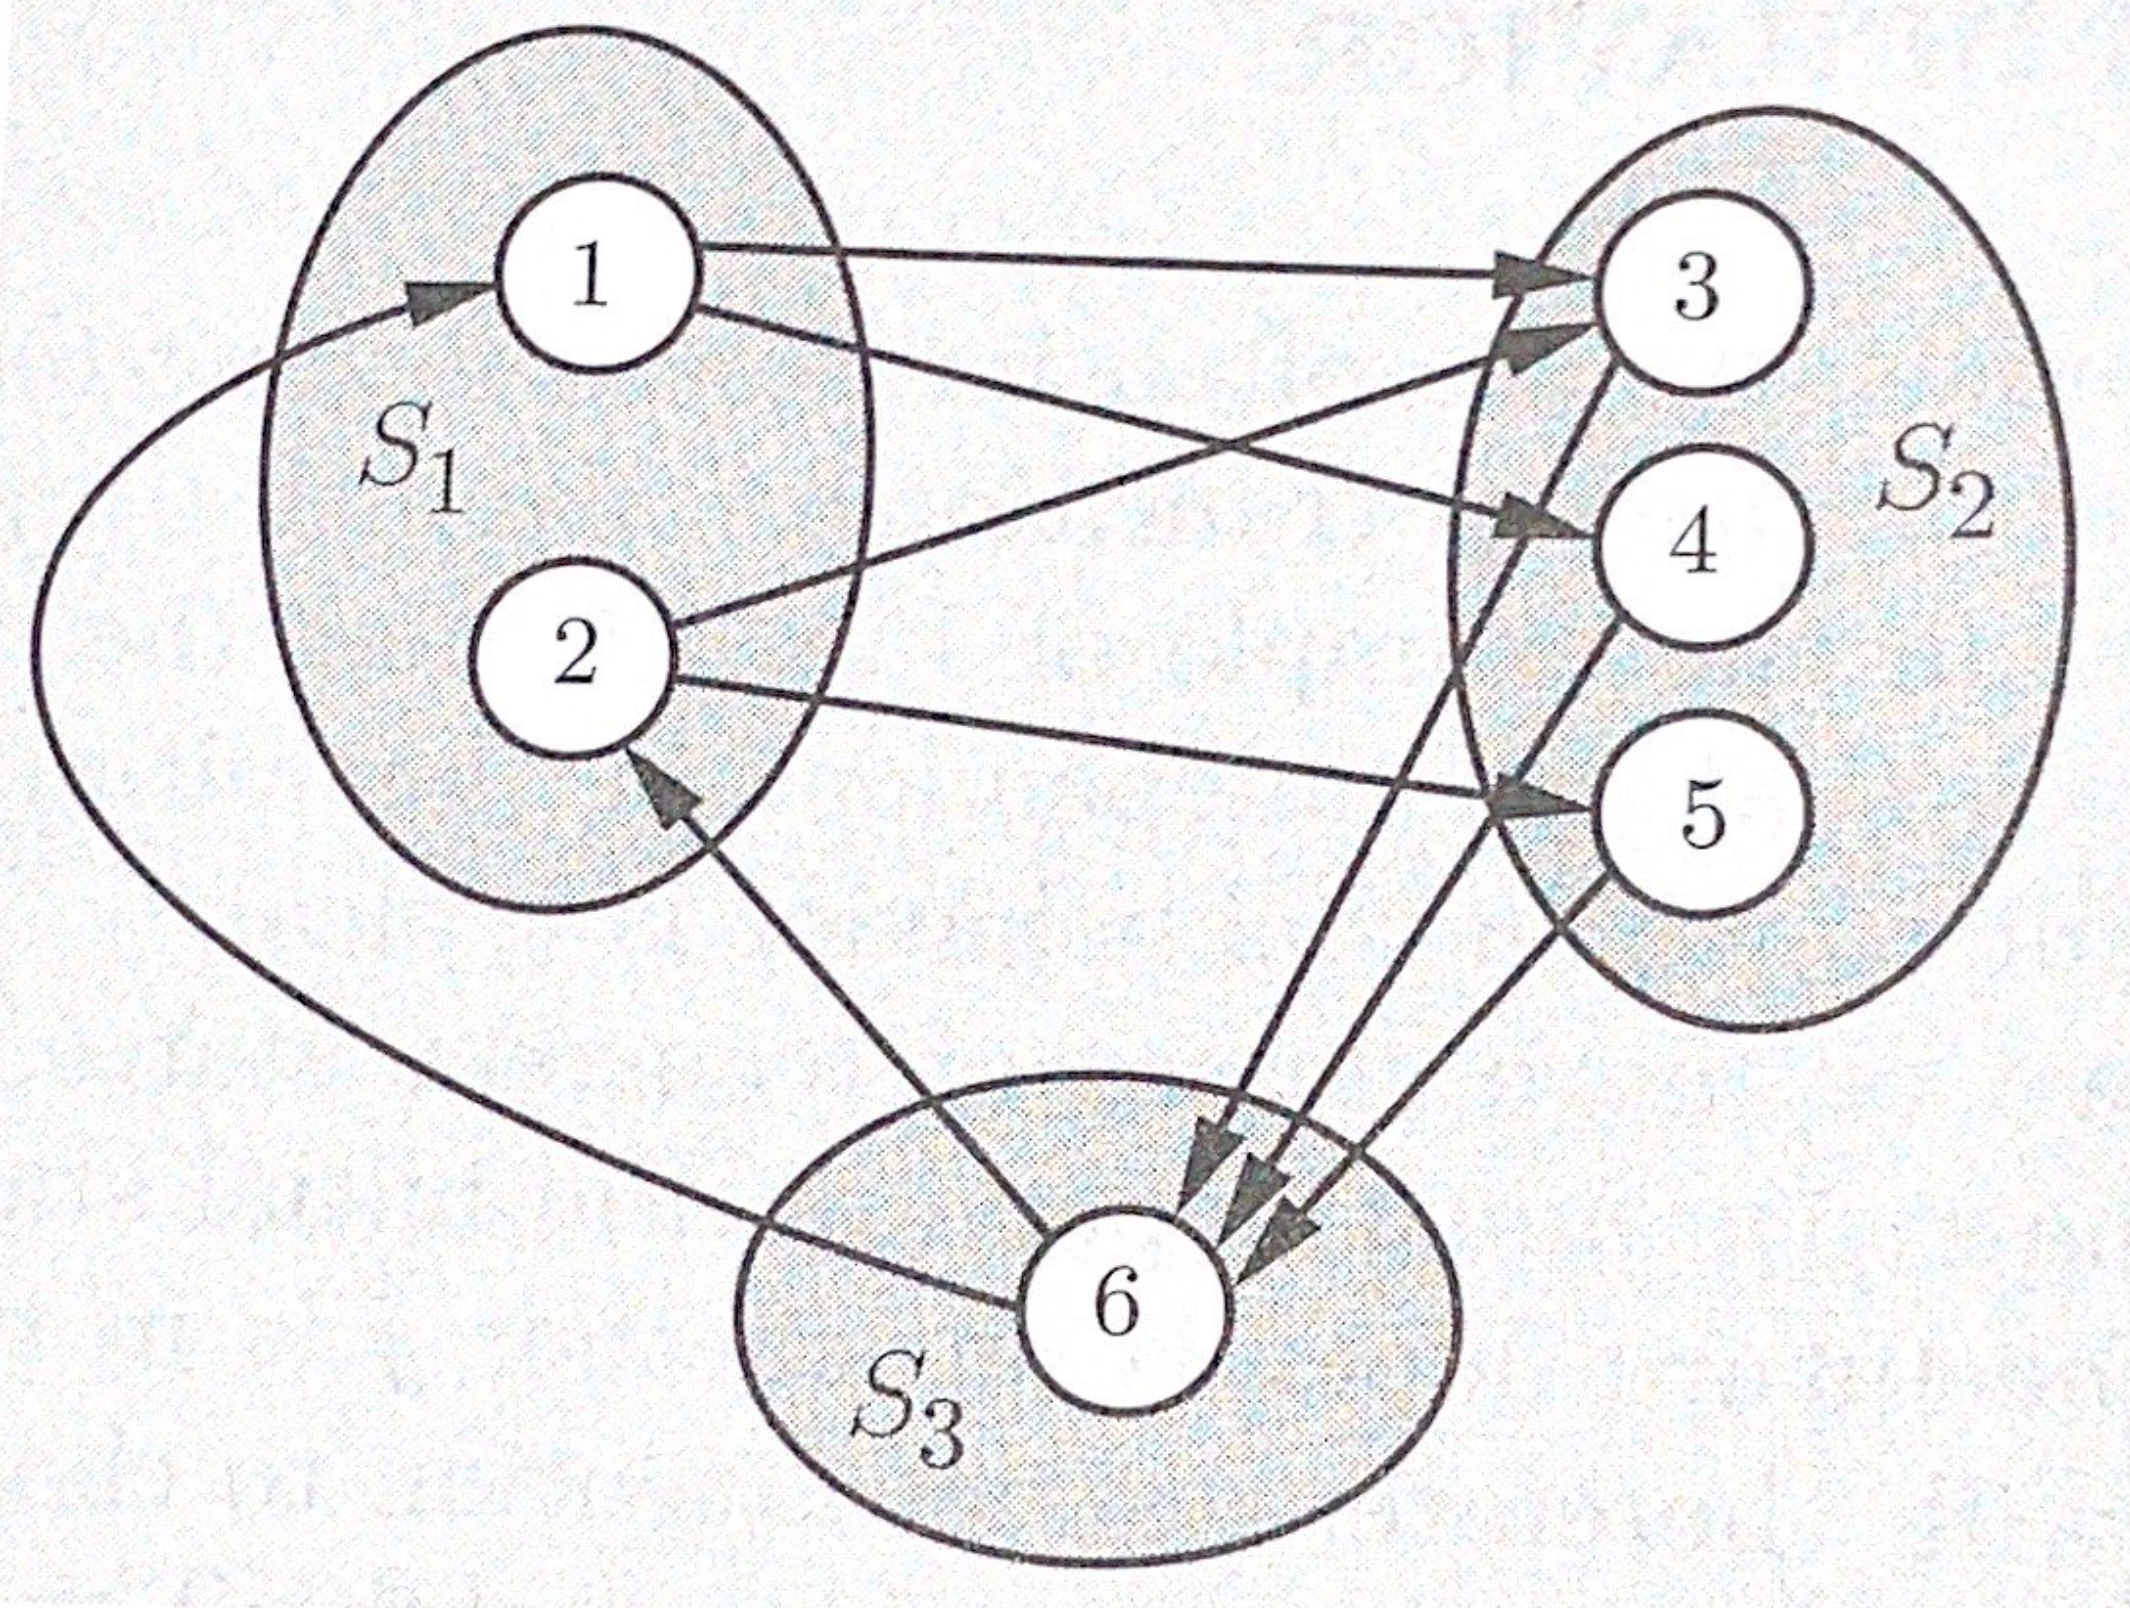
\includegraphics[width=0.2\columnwidth]{L9_periodic_1.png}
  \hspace{1cm}
  \includegraphics[width=0.15\columnwidth]{L9_periodic_2.png}
  \hspace{1cm}
  \includegraphics[width=0.23\columnwidth]{L9_periodic_3.png}

\vspace{-0.3cm}
  \plitemsep 0.05in
  \bci
  
\item<2-> \defi A recurrent class  is said to be \redf{periodic}, if
  its states can be grouped in $d >1$ disjoint subsets $S_1, \ldots,
  S_d$ so that all transitions from $S_k$ lead to $S_{k+1}$ (or to
  $S_1$ if $k=d$). We call $d$ the \redf{period} of the recurrent class. 
  
  % \mypic{0.3}{L9_periodic_1.png}
  % \mypic{0.3}{L9_periodic_2.png}
  % \mypic{0.3}{L9_periodic_3.png}
  
  
\item<3-> A recurrent class that is not periodic (i.e., period $d=1$) is said to be
  \redf{aperiodic}.
  

\item<4-> For any state $i$ in the $d$-period recurrent class,
  \redf{$r_{ii}(n)=0$}, whenever $n$ is not divisible by $d$, where $d$ is the greatest
  integer with this property. 

\item<5-> Often, it is not easy to see some MC is periodic or
  not. But, one easy way is to check whether there exists a
  self-transition or not. \bluef{An MC with a self-transition must be
  aperiodic.} 

  
  %\item<3-> A recurrent class that is not periodic is said to be
  %   \redf{aperiodic}.
  %   \bci
  % \item The class is aperiodic if and only if there exists a time $n$
  %   such that $r_{ij}(n) > 0,$ for all $i,j.$
  %   \eci
  
  \eci
  
\end{frame}

% %%%%%%%%%%%%%%%%%%%%%%%%%%%%%%%%%%%%%%%%%%%%%%%%%%%%%%
% \begin{frame}{Periodicity (2)}


% \centering
% 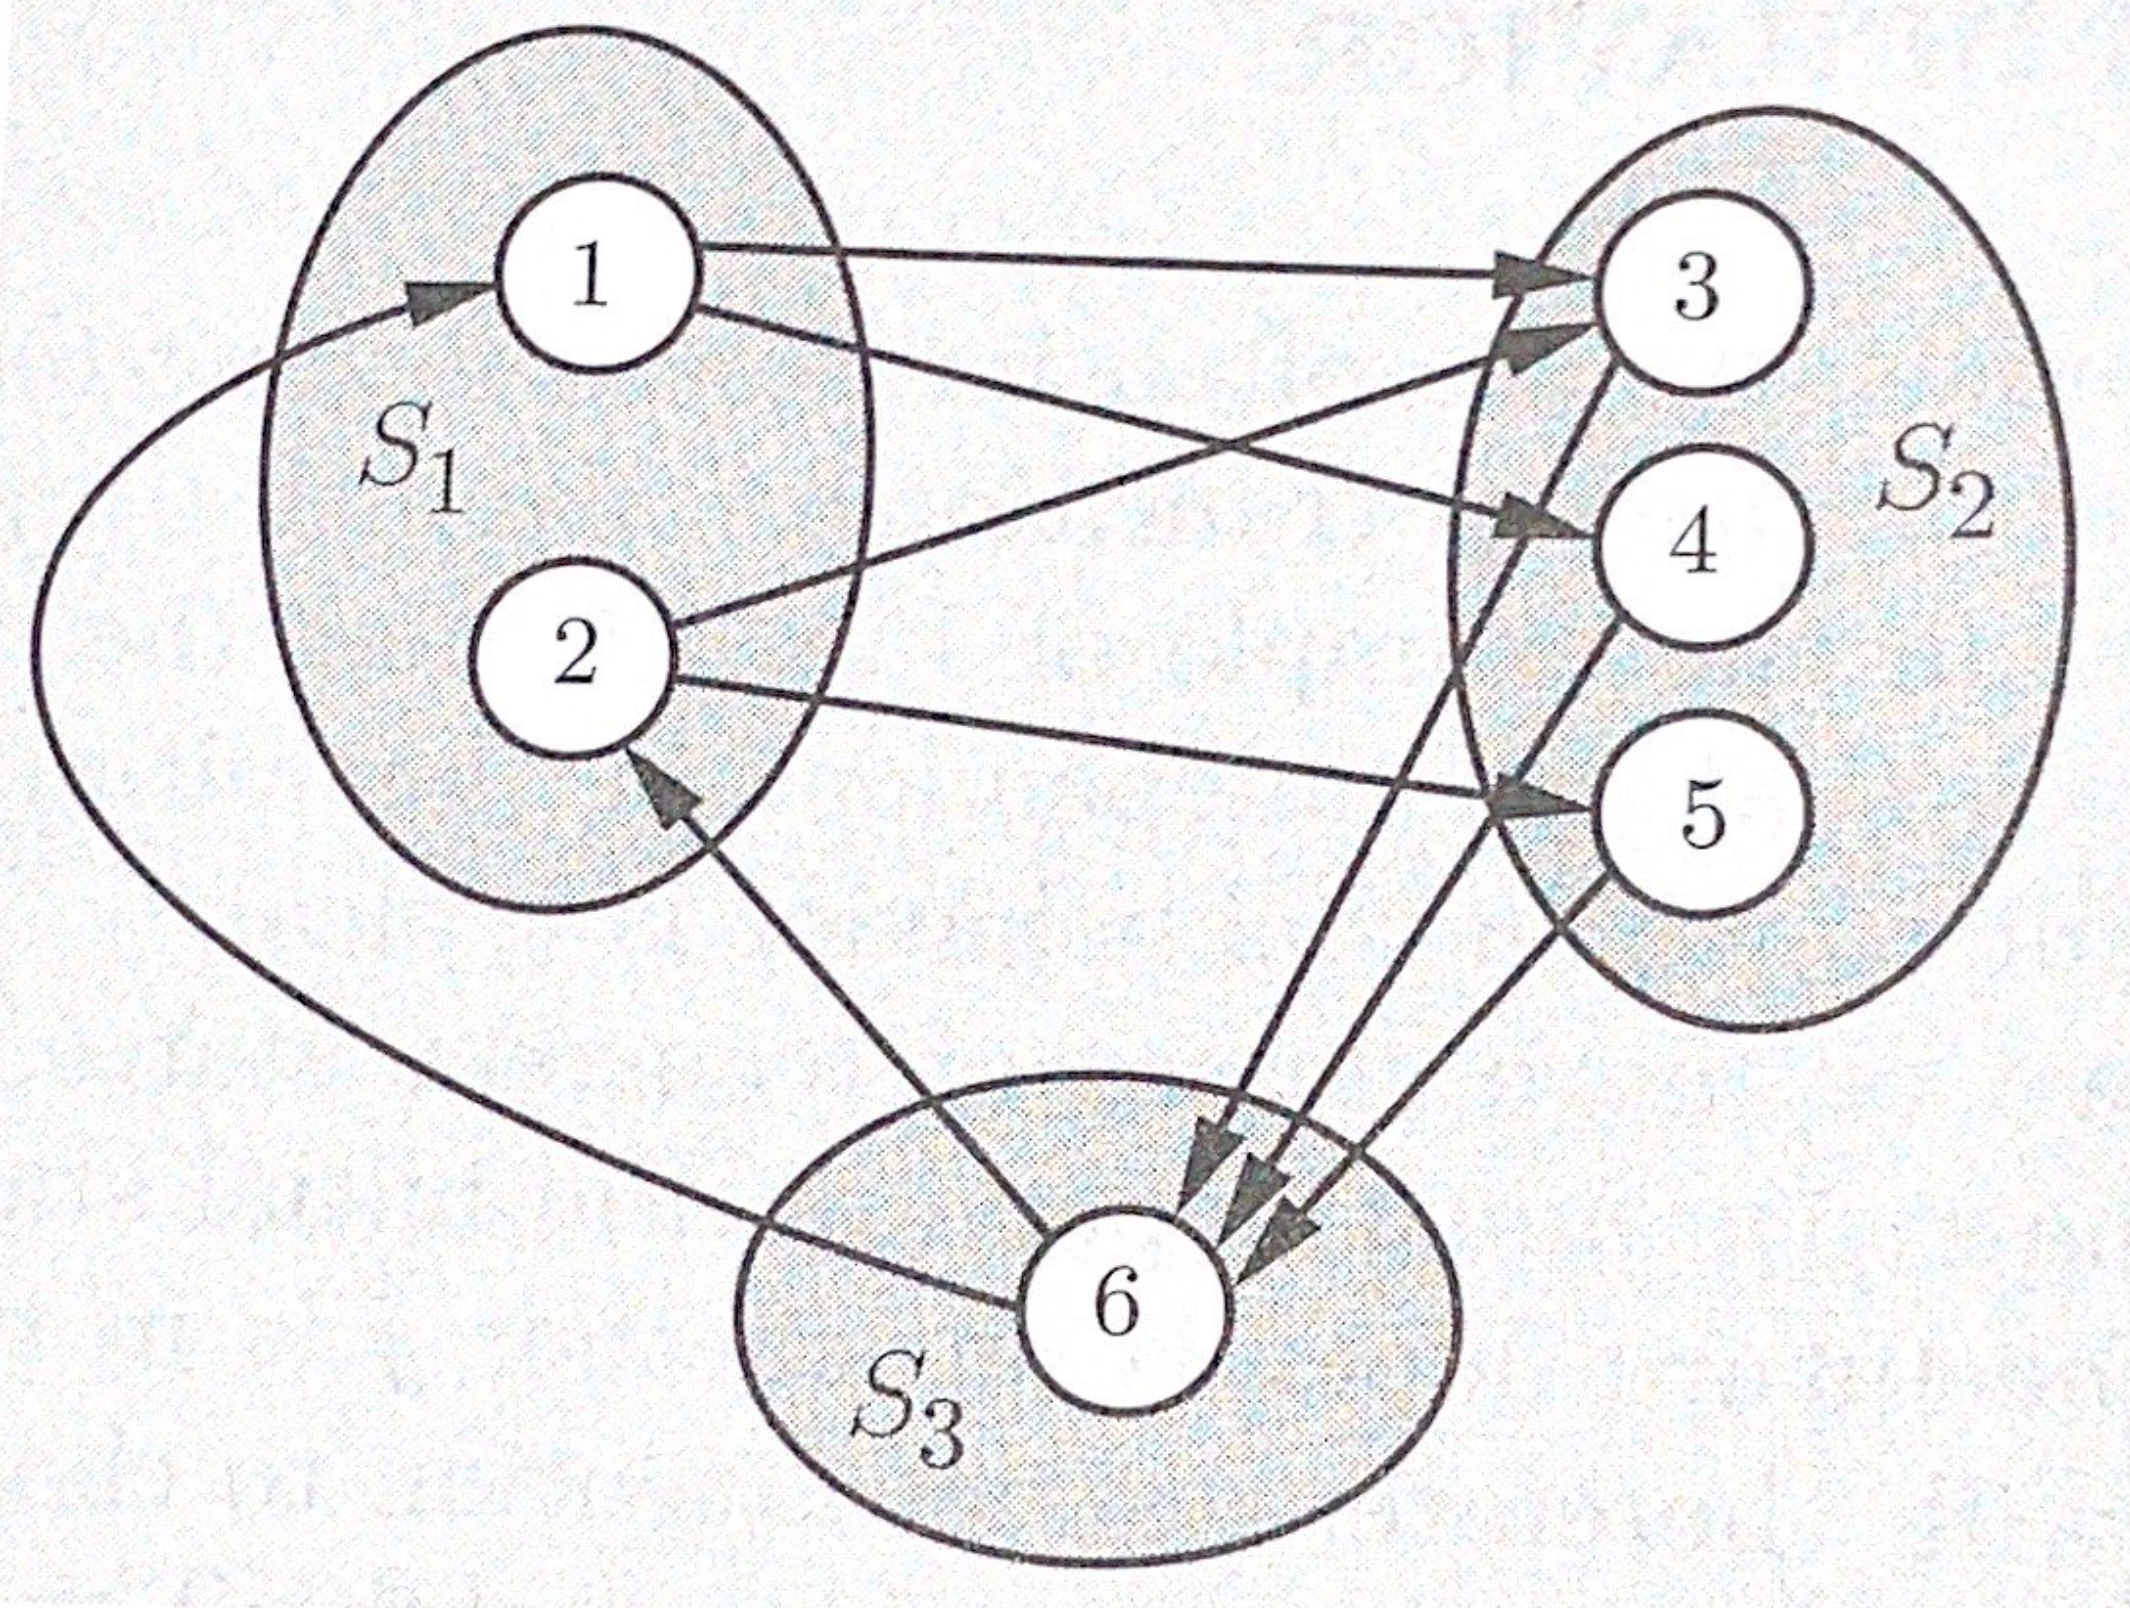
\includegraphics[width=0.2\columnwidth]{L9_periodic_1.png}
% \hspace{1cm}
% \includegraphics[width=0.15\columnwidth]{L9_periodic_2.png}
% \hspace{1cm}
% \includegraphics[width=0.23\columnwidth]{L9_periodic_3.png}


% \plitemsep 0.1in
% \bci

% \item For any state $i$ in the $d$-period recurrent class,
%   $r_{ii}(n)=0,$
%   whenever $n$ is not divisible by $d$, where $d$ is the greatest
%   integer with this property. 


% \item Given a periodic recurrent class, a time $n,$ and a
%   state $i$ in the class, there must exist one ore more states $j$ for
%   which $r_{ij}(n) =0.$
  
% \item The class is aperiodic if and only if there exists a time $n$
%   such that $r_{ij}(n) > 0,$ for all $i,j.$
  
%   \eci
  
% \end{frame}



%%%%%%%%%%%%%%%%%%%%%%%%%%%%%%%%%%%%%%%%%%%%%%%%%%%%%%
\section{L8(4)}
\begin{frame}{Roadmap}

{\Large Markov Chain}


  \plitemsep 0.1in

\bce[(1)]


%\item \redf{Markov Chain}

\item \grayf{Definition, Transition Probability Matrix, State Transition Diagram}

\item \grayf{$n$-step Transition Probability}

\item \grayf{Classification of States}

\item \redf{Steady-state Behaviors and Stationary Distribution}

\item \grayf{Transient Behaviors}



\ece 

\end{frame}


%%%%%%%%%%%%%%%%%%%%%%%%%%%%%%%%%%%%%%%%%%%%%%%%%%%%%%
\begin{frame}{$n$-step transition prob.: $r_{ij}(n)$ for large $n$}

\mytwocols{0.6}
{
\bci
\item<2-> \small Convergence \redf{irrespective of} the start state
\eci


%\medskip
\vspace{-0.3cm}
\mypic{0.95}{L9_inftysteps1.png}
}
{
\bci
\item<3-> \small Convergence \redf{depending on} the start state
\eci


%\medskip
\vspace{-0.3cm}
\mypic{0.95}{L9_inftysteps2.png}
}

\onslide<4->{\redf{(Q)} Under what conditions, convergence occurs,
  \redf{independent of} the start state? If
  so, how does it depend on the start state and the shape of the MC?}

\end{frame}


%%%%%%%%%%%%%%%%%%%%%%%%%%%%%%%%%%%%%%%%%%%%%%%%%%%%%%
\begin{frame}{Steady-state behavior: Why Impotant?}

\mytwocols{0.7}
{
\plitemsep 0.1in

\bci
\item $r_{ij}(n) \xrightarrow{n \rightarrow \infty} \pi_j$, for some $\pi_j \le 1$?

\item<2-> \redf{Interpretation.}
\mycolorbox{
\centering
  $\pi_j \approx \cprob{X_n = j}$ for large $n$
}

\item<3-> After running the MC for a long time, we see
  how long the MC will stay at which state on average. 

\item<4-> Helps in understanding how this MC behaves. 

  \eci

}
{
\mypic{0.8}{L9_machine_std.png}

\centering
$\pi_{\text{working}} = \alpha$

\medskip
$\pi_{\text{broken}} = \beta$

}

\end{frame}


%%%%%%%%%%%%%%%%%%%%%%%%%%%%%%%%%%%%%%%%%%%%%%%%%%%%%%
\begin{frame}{Steady-state behavior: Convergence Condition}

\mytwocols{0.7}
{
\plitemsep 0.1in

\bci
\item $r_{ij}(n) \xrightarrow{n \rightarrow \infty} \pi_j$, for some $\pi_j \le 1$?

\item Convergence occurs, \redf{independent of} the starting state, if:
\bce[\bf C1.]
\item<2-> Only a \redf{single recurrent class}
\item<4-> such recurrent class is \redf{aperiodic}
\ece

\item<3->[\small\bf C1.] {\small For the case of multiple recurrent classes, one stays at the class including the starting state.} 

\item<5->[\small \bf C2.] {\small Divergent behavior for periodic recurrent classes. }

\eci

}
{
\vspace{-0.4cm}
\centering
\onslide<3->{
\mypic{0.8}{L9_class_ex.png}
\vspace{-0.4cm}
{\small (a) multiple recurrent classes}
}

\onslide<5->{
\mypic{0.7}{L9_periodic_ex.jpg}
\vspace{-0.4cm}
{\small (b) single recurrent, but periodic class}
}
}

\end{frame}


%%%%%%%%%%%%%%%%%%%%%%%%%%%%%%%%%%%%%%%%%%%%%%%%%%%%%%
\begin{frame}{Steady-state Convergence Theorem}

  \redf{(Q)} How to easily compute $(\pi_1, \pi_2, \ldots, \pi_m)$
  rather than taking the limit?
  
\plitemsep 0.1in
\bci
\item<2-> If $r_{ij}(n) \xrightarrow{n \rightarrow \infty} \pi_j$, for
  some $\pi_j \le 1,$ from Chapman-Kolmogorov equation, 
\aleq{
\onslide<2->{r_{ij}(n) &= \sum_{k=1}^m r_{ik}(n-1) p_{kj} \imp} \onslide<3->{\redf{\pi_j = \sum_{k=1}^m \pi_k p_{kj}}} \qquad \onslide<4->{\text{\bluef{(Balance equation)}}}
}

\item<5-> $
\displaystyle \redf{\sum_{i=1}^m \pi_i = 1}
$: \bluef{(Normalization equation)}

\item<6-> Balance eqn. + Normalization eqn. $\imp$  Finding the steady-state probabilities $\{\pi_i \}.$
  \bci
  \item Solving linear equations
%  \item If we let $\mat{\pi} = (\pi_1, \ldots, \pi_m).$ Solve $\mat{\pi} = \mat{\pi}\mat{P}.$
    \eci
  
\eci


\end{frame}


%%%%%%%%%%%%%%%%%%%%%%%%%%%%%%%%%%%%%%%%%%%%%%%%%%%%%%
\begin{frame}{Long-term Frequency Interpretation}

\mytwocols{0.7}
{
\small
  \plitemsep 0.1in
\bci

\item Probability: often interpreted as the \redf{relative frequencies} out
  of many independent trials

\item   $\displaystyle \pi_j = \lim_{n \rightarrow \infty}
  \frac{v_{ij}(n)}{n},$ where $v_{ij}(n)$ is the expected number of
  visits to state $j$ up to the first $n$ transitions

\item In other words, $\pi_j$: long-term \redf{expected fraction
    of time} that the MC is at the state $j.$

\item $\pi_j p_{jk}$: the long-term expected \redf{fraction of transitions}
  that move the state \redf{from $j$ to k.}



  \eci

}
{
\small
     \plitemsep 0.1in
 \bci
\item Balance equation: $\bluef{\sum_{k=1}^m \pi_k p_{kj}} = \orangef{\pi_j}$

\bci
\item  \orangef{The expected frequency of visits to $j$}
  =

  \bluef{The sum of the expected frequencies of transitions that lead to $j.$}
\eci

 \eci
  \vspace{-0.2cm}
\mypic{0.6}{L9_longtermfrequency.png}
}

\end{frame}


%%%%%%%%%%%%%%%%%%%%%%%%%%%%%%%%%%%%%%%%%%%%%%%%%%%%%%

\begin{frame}{Example 1}

\plitemsep 0.1in
\bci

\item A two-state MC with:
  $
  \begin{nmat}
    0.8 & 0.2 \cr
    0.6 & 0.4 
  \end{nmat}
  $

\item (Balance equation) 
\aleq{
  \pi_1 &= \onslide<2->{\pi_1 p_{11} + \pi_2 p_{21} = 0.8\pi_1 + 0.6\pi_2,} \cr
  \pi_2 &= \onslide<3->{\pi_2 p_{22} + \pi_1 p_{12} = 0.4 \pi_2 + 0.2 \pi_1} 
}
\item (Normalization equation) \onslide<4->{$\pi_1 + \pi_2 = 1$}

\item Steady-state probabilities: \onslide<5->{$\pi_1 = 0.25$, $\pi_2 = 0.75.$}

\eci
\end{frame}


%%%%%%%%%%%%%%%%%%%%%%%%%%%%%%%%%%%%%%%%%%%%%%%%%%%%%%
\begin{frame}{Stationary Distribution}

\footnotetext{stationary: not moving or not intended to be moved.}
\plitemsep 0.1in
\bci

\item<2-> $\{ \pi_j \}$ is also called a \redf{stationary distribution}. Why?

\item<3-> \redf{Distribution}, because $\sum_{j=1}^m \pi_j =1.$

\item<4-> \redf{Stationary}, because, if you choose the initial state
  according to $\{\pi_j \},$ then for any $j \in \{1, \ldots, m \}$ 
\aleq{
\cprob{X_0 = j} = \pi_j \xrightarrow{\text{total prob. theorem}}
\onslide<5->{\orangef{\cprob{X_1 = j}} = \sum_{k=1}^m \cprob{X_0=k}
  p_{kj} =} \onslide<6->{\sum_{k=1}^m \pi_k p_{kj} 
= \orangef{\pi_j}}
}

\bci
\item<7-> Similarly, we have $\cprob{X_n = j} = \pi_j$, for all $n$ and $j.$

\item<8-> If the initial state is chosen according to $\{\pi_j \},$ the state at any future time will have the same distribution (i.e., the distribution does not change over time). 

\eci

\item<9-> We say that "the limiting distribution (steady-state
  distribution) is equal to to the stationary distribution"

\eci


\end{frame}



%%%%%%%%%%%%%%%%%%%%%%%%%%%%%%%%%%%%%%%%%%%%%%%%%%%%%%
\begin{frame}{Example 2}

  \mytwocols{0.75}
  {
    \small
    \plitemsep 0.1in
    \bci
    
  \item An absent-minded professor: two umbrellas from home to office
    and back.

  \item<2-> If it rains and an umbrella is available, she takes it. If it
    is not raining, she always forgets to take an umbrella. 
    
\item<3-> Suppose that it rains w.p. $0< p< 1$ each time when she commutes,
  independent of other times.  

\item<4-> \redf{(Q)} What is the steady-state probability that she gets
  wet during a commute?

\item<5-> \bluef{(Hint)} If you think that this can be modeled by a MC,
  think about what should be chosen as states. What is changing over
  time?   \hfill   \lecturemark{VIDEO PAUSE}
  \eci
}
{
  \small
  \plitemsep 0.03in
  \bci
\item<6-> state $i \in \{0,1,2\}$: $i$ umbrellas available in her location.
\item<7-> Transition diagram
\onslide<8->{\mypic{0.8}{L9_umbrella.png}}
\item<9-> Single recurrent class and aperiodic  
\item<10-> Balance and normalization equation
\vspace{-0.2cm}
  \aleq
  {
    \pi_0 &= \onslide<11->{(1-p)\pi_2}, \quad \pi_1 = \onslide<11->{(1-p)\pi_1 + p \pi_2} \cr
    \pi_2 &= \onslide<11->{\pi_0 + p\pi_1}, \quad \pi_0 + \pi_1 + \pi_2 = 1
  }
\item<12-> $\pi_0 = \frac{1-p}{3-p}$, $\pi_1 = \frac{1}{3-p},$
  $\pi_2 = \frac{1}{3-p}.$ 
\item <13-> The answer is $p \times \pi_0.$
  \eci    
}
\end{frame}


%%%%%%%%%%%%%%%%%%%%%%%%%%%%%%%%%%%%%%%%%%%%%%%%%%%%%%
\begin{frame}{Example 3: Random Walk with Reflecting Barriers}

    \plitemsep 0.05in
    \bci
    
  \item A person walks along a straght line, and at each time, moves
    right w.p. $b$ and moves left w.p. $1-b$.

  \item<2-> Starts in one of the positions $1, 2, \ldots, m.$

  \item<3->     If he reaches position 0 (or position $m+1$), his step is instantly
    reflected back to position 1 (or position $m$, respectively). 
    \eci
%\vspace{-0.5cm}

\onslide<4->{\mypic{0.6}{L9_bd_2.png}}

\end{frame}

%%%%%%%%%%%%%%%%%%%%%%%%%%%%%%%%%%%%%%%%%%%%%%%%%%%%%%
\begin{frame}{Example 4: Queueing}

  \mytwocols{0.5}
  {
    \small
    \plitemsep 0.03in
    \bci
    
  \item Customers arrive at the supermarket counter. If there are some
    customers at the counter, then new customers should wait in a line
    whose capacity is $m.$

  \item<2-> If there are $m$ customers, then new
    customer cannot wait in the line, and is discarded. 


  \item<3-> We assume discrete time slots. We assume that at each time
    slot,  exactly one of the followings (a), (b), and (c) occurs

    \eci
  }
  {
  \small
  \plitemsep 0.03in
  
    \bce[(a)]
  \item<4-> A new cutomer arrives w.p. $b >0$
  \item<5-> One existing customer at the counter leaves w.p. $d >0.$ If
    there are no customers, nothing happens.  
  \item<6-> No new customer and no existing customer leaves w.p. $1-b-d$,
    if there is at least one customer at the counter and w.p. $1-b$
    otherwise. 

%  \item[$\bullet$] Draw the state transition diagram

    \ece
}

\vspace{-0.6cm}
\onslide<7->{\mypic{0.55}{L9_bd_3.png}}

\end{frame}

%%%%%%%%%%%%%%%%%%%%%%%%%%%%%%%%%%%%%%%%%%%%%%%%%%%%%%
\begin{frame}{Birth-Death Process (1)}

  \plitemsep 0.07in
  \bci
  
\item<2-> A special type of Markov chain where the states are \redf{linearly arranged}
  and transitions can only occurs to a \redf{neighboring} state. 

\item<3-> Birth and Deadth
  \aleq{
   \redf{b_i} &= \cprob{X_{n+1} = i+1 | X_n = i}, \quad \text{\redf{birth} probability at state $i$}\cr
    \bluef{d_i} &= \cprob{X_{n+1} = i-1 | X_n = i}, \quad \text{\bluef{death} probability at state $i$}
  }
  
  \eci
  
\vspace{-0.5cm}
\onslide<3->{\mypic{0.7}{L9_bd_1.png}}
\end{frame}

%%%%%%%%%%%%%%%%%%%%%%%%%%%%%%%%%%%%%%%%%%%%%%%%%%%%%%
\begin{frame}{Birth-Death Process (2)}


\mytwocols{0.75}
{
\small
  \plitemsep 0.03in
  \bci
  
\item State transition diagram
\vspace{-0.4cm}
\mypic{0.95}{L9_bd_1.png}

\item<2-> Balance eqn at state 0
  \aleq{
    \pi_0 (1-b_0) + \pi_1 d_1 = \pi_0 \leftrightarrow \onslide<3->{\orangef{\pi_0 b_0 =
    \pi_1 d_1}}
  }

\item<4-> Balance eqn at state 1  
  \aleq{
&    \pi_0 b_0 + \pi_1 (1-b_1 - d_1) + \pi_2 d_2 = \pi_1 \cr
&\leftrightarrow \onslide<5->{\pi_1 d_1 + \pi_1(1-b_1-d_1) + \pi_2 d_2 = \pi_1} \cr
&\leftrightarrow \onslide<6->{\orangef{\pi_1 b_1 = \pi_2 d_2}}
}
\eci
}
{
\small
  \plitemsep 0.07in
  \bci
\item<7-> By induction, we have the following: called \redblank{8}{local balance equation}:
  \mycolorbox{
\onslide<8->{    $\pi_i b_i = \pi_{i+1} d_{i+1}$, $i=0,1, \ldots, m-1$}
  }

\item<9-> Using the above local balance eqn,
  \aleq{
    \pi_i = \pi_0 \frac{b_0 b_1 \cdots b_{i-1}}{d_1 d_2 \cdots d_i}, \quad
    i=1, \ldots, m
  }

\item<10-> Using the above and $\sum \pi_i =1,$ we can easily compute the $[\pi_i].$


\item<11-> Examples 3 and 4 are the special cases of birth-death
  process. So, please compute the steady-state probabilities for both
  examples as your homeworks.  

  \eci
 
}
  


\end{frame}





%%%%%%%%%%%%%%%%%%%%%%%%%%%%%%%%%%%%%%%%%%%%%%%%%%%%%%
\section{L8(5)}
\begin{frame}{Roadmap}

{\Large Markov Chain}


  \plitemsep 0.1in

\bce[(1)]


%\item \redf{Markov Chain}

\item \grayf{Definition, Transition Probability Matrix, State Transition Diagram}

\item \grayf{$n$-step Transition Probability}

\item \grayf{Classification of States}

\item \grayf{Steady-state Behaviors and Stationary Distribution}

\item \redf{Transient Behaviors}

\ece 

\end{frame}


%%%%%%%%%%%%%%%%%%%%%%%%%%%%%%%%%%%%%%%%%%%%%%%%%%%%%%
\begin{frame}{Absorption Probability}

\mytwocols{0.5}
{
\small
\plitemsep 0.03in
\bci
\item<1-> \defi A state $k$ is \redf{absorbing,} if
$p_{kk}=1,$ and $p_{kj}=0$ for all $j\neq k.$

\onslide<2->{- states 1 and 6 are absorbing}

\item<3->[\redf{(Q)}] For a fixed absorbing state $s,$ the probability $a_i$ of reaching $s$, starting from a transient state $i$?

%\item Interested in the transient behavior of a MC.

\item<4-> Fix $s=6.$ 
\vspace{-0.3cm}
\aleq{
a_1 &=0, \quad a_6 =1 \cr
a_2 &= 0.2a_1 + 0.3a_2 + 0.4a_3 + 0.1 a_6 \cr
a_3 &= 0.2 a_2 + 0.8 a_6
}
\eci
}
{
\vspace{-0.4cm}
\onslide<4->{\mypic{0.65}{L9_absorption_ex1.png}}
\vspace{-0.6cm}
\onslide<5->{\mypic{0.7}{L9_absorption_ex2.png}}
}

\small
\bci
\item<5-> \redf{(Q)} What if there are some non-absorbing recurrent state?

\item<6-> Convert it into the one only with absorbing recurrent states (from (a) to (b)).
\eci

% \onslide<5->{\redf{(Q)} What if there are some non-absorbing recurrent state? }

% \onslide<6->{- Convert it into the one only with absorbing recurrent states (from (a) to (b)).}

\footnotetext{The notation $a_i$ should have dependence on $s,$ but we omit it for simplicity.}
\end{frame}

%%%%%%%%%%%%%%%%%%%%%%%%%%%%%%%%%%%%%%%%%%%%%%%%%%%%%%
\begin{frame}{Expected Time to Any Absorbing State}

\mytwocols{0.2}
{
\small
\plitemsep 0.1in
\bci

\item[\redf{(Q)}] Starting from a transient state $i,$ expected number of transitions $\mu_i$ until absorption to any absorbing state?
% \aleq{
% \mu_i = \expect{\text{\# of transitions until absorption, starting from $i$}}
% }
\eci
}
{
\centering
\vspace{-0.5cm}
\mypic{0.75}{L9_spiderfly_onlyfigure.png}
% \mypic{0.8}{L9_absorption_ex2.png}
}

\small
\plitemsep 0.1in
\bci
\item<2-> Spider-fly example
\aleq{
\mu_1 &= \mu_4 =0 \quad \text{(for recurrent states)}\cr
\mu_2 &= \redf{1+} 0.4\mu_2 + 0.3 \mu_3, \quad \mu_3 = \redf{1 +} 0.3\mu_2 + 0.4\mu_3 \quad \text{(for transient states)}
}

\item<3-> For generalized description, please see the textbook (pp. 367). 

\eci

\end{frame}

%%%%%%%%%%%%%%%%%%%%%%%%%%%%%%%%%%%%%%%%%%%%%%%%%%%%%%
\begin{frame}{Expected time to a particular recurrent state $s$}

- Assume a single recurrent class
\myvartwocols{0.2}{0.7}{0.29}
{
\small
\plitemsep 0.1in
\bci
\item<2->[\redf{(Q)}] \bluef{First passage time.} Starting from a $i,$ expected number of transitions $t_i$ to reach $s$ for the first time?

\item<4->[\redf{(Q)}] \bluef{First recurrence time.} Starting from a $s,$ expected number of transitions $t_s^\star$ to reach $s$ for the first time?

% \aleq{
% \mu_i = \expect{\text{\# of transitions until absorption, starting from $i$}}
% }
\eci
}
{
\vspace{-0.2cm}
\mypic{0.8}{L9_passage_ex.png}
% \mypic{0.8}{L9_absorption_ex2.png}
}
 \small
 \plitemsep 0.01in
 \bci
 \item<3-> Mean first passage time from 2 to 1
\vspace{-0.2cm}
   \aleq{
 t_1 &= 0 \cr
 t_2 &= 1+ p_{21}t_1 + p_{22}t_2 = 1+ 0.4 t_2 \imp t_2 = 5/3
 }
 \item<5-> Mean first recurrence time from 1 to 1
\vspace{-0.2cm}
   \aleq{
 t_1^\star &= 1+ p_{11}t_1 + p_{12}t_2 = 1+ 0 + 0.2\frac{5}{3} = \frac{4}{3}
 }

\item<6-> For generalized description, please see the textbook (pp. 368)
 \eci

\footnotetext{The notation $t_i$ should have the dependence on $s$, but we omit it for simplicity.}

\end{frame}

%%%%%%%%%%%%%%%%%%%%%%%%%%%%%%%%%%%%%%%%%%%%%%%%%%%%%%
\begin{frame}{}
\vspace{2cm}
\LARGE Questions?

\end{frame}

%%%%%%%%%%%%%%%%%%%%%%%%%%%%%%%%%%%%%%%%%%%%%%%%%%%%%%
\begin{frame}{Review Questions}

\bce[1)]
\item Why do you think Markov chain (MC) is important?

\item What is the Markov property and its meaning? What's the key difference of MC from Bernoulli processes?

\item What are the limiting distribution and the stationary distribution of MCs?

\item How are you going to  compute the stationary distribution, if you are given a transition probability matrix?

\item What are recurrent and transient states in MC?


\ece

\end{frame}



% %%%%%%%%%%%%%%%%%%%%%%%%%%%%%%%%%%%%%%%%%%%%%%%%%%%%%%
% \begin{frame}{Example}

% \plitemsep 0.1in

% \bci 
% \item Let $\set{E} = \{\ldots,-2,-1,0,1,2,\ldots \},$. Initially, $X_0 =
%   0,$ and $\forall n \leq 0,$
% \aleq{
%     \prob{X_{n+1}& = X_n +1 \vert X_n} = \prob{X_{n+1}= X_n-1 \vert X_n}
%     = 1/2. 
% }
  
% \item Draw transition diagram.
% \vspace{2.5cm}

% \item Check whether the above is Markov chain or not.

% \eci 
% \end{frame}

%%%%%%%%%%%%%%%%%%%%%%%%%%%%%%%%%%%%%%%%%%%%%%%%%%%%%%
% \begin{frame}{Definitions}

% \plitemsep 0.1in

% \bci 
% \item \defi Given HMC with transition matrix $P,$ $P^n$ is the $n$-step
%   transition matrix, i.e., $P^n=[p_{ij}(n)],$ where $p_{ij}(n)=$
%   probability of visiting $j$ in the $n$-step starting from $i$.

% \item \defi Node $i$ communicates with $j$ if there exist $n_1,n_2\geq
%   0,$ s.t. $p_{ij}(n_1)>0$ and $p_{ji}(n_2)>0$, denoted by $i
%   \leftrightarrow j.$

% \item \defi Communication defines ``equivalence class'' of HMC: (i) if
%   $i\leftrightarrow j,$ and $j \leftrightarrow k,$ then $i
%   \leftrightarrow k,$ and (ii) $i \leftrightarrow i$ (since $p_{ii}(0) =
%   1$).

% \item \defi A Markov chain is called {\red irreducible} if there is only one
%   communication class. {\blue Any state can be reachable starting from
%     any other state.}

% \item An example of a Markov chain that is not irreducible?

% \item Henceforth, we only consider a irreducible Markov chain.

% \eci 
% \end{frame}

% %%%%%%%%%%%%%%%%%%%%%%%%%%%%%%%%%%%%%%%%%%%%%%%%%%%%%%
% \begin{frame}{Period}

% \plitemsep 0.1in

% \bci 
% \item The period of $d(i)$ of state $i \in \set{E}$ is defined by 
% $    d(i) = gcd\{n: p_{ii}(n) >0\}.$


% \item We call $i$ {\red periodic} if $d(i)>1$ and {\red aperiodic} if $d(i)=1.$

% \item An irreducible HMC is called {\red aperiodic} if all of its period is
%   aperiodic.

% \item Period is a class property

% \bci
% \item If $i$ and $j$ communicate, then
%   they have the same period. 
 
% \item Thus, it suffices to check one state's
%   aperiodicity for a irreducible Markov chain, if you want to check the
%   aperiodicity of the entire Markov chain. 

% % \item \redf{Proof.}  As $i \leftrightarrow j,$ there exists integers $N,M,$ such that
% % $p_{ij}(M)>0$ and $p_{ji}(N) >0.$ For any $k \geq 1,$
% % \aleq{
% %   p_{ii}(M+nk +N) \geq p_{ij}(M) (p_{jj}(k))^n p_{ji}(N). \text{\qed}
% % }
% % Thus, for any $k\geq 1,$ such that $p_{jj}(k) >0,$ we have
% % $p_{ii}(M+nk+N) >0$ for all $n\geq 1.$ Then, $d_i$ divides $M+nk+_N$ for
% % all $n\geq 1,$ and in particular, $d_i$ divides $k.$ Thus, $d_i$ divides
% % all $k,$ such that $p_{jj}(k) >0,$ in particular, $d_i$ divides $d_j.$
% % By symmetry, $d_j$ divides $d_i.$ Thus, $d_i = d_j.$

% \eci

% \item Example. Two states 1 and 2. $p_{12} = 1$ and $p_{21} = 1.$

% \eci 
% \end{frame}

% %%%%%%%%%%%%%%%%%%%%%%%%%%%%%%%%%%%%%%%%%%%%%%%%%%%%%%
% \begin{frame}{Recurrence}

% \plitemsep 0.05in

% \bci 
% \item \defi Let $T_i = \min \{k\geq 1 \vert X_{k}=i \}.$ Then, mentioned
%   earlier, $T_i$ is a
%   stopping time. State $i$ is called {\red recurrent} if $\probi{i}{T_i} 
%   \triangleq \prob{T_i < \infty | X_0=i} = 1,$ otherwise called {\red transient}.

% \item Staring from a state $i$, I will return to the state $i$ within a
%   finite time with probability 1.

% \item Let $f_{ii}^{(n)} = \prob{T_i = n \mid X_o = i},$ which is the
%   probability that the first return time from $i$ to $i$ is $n.$ Then,
%   from the definition {\red recurrent} if $\sum_{n=1}^\infty f_{ii}^{(n)} = 1,$ and {\red transient} if $\sum_{n=1}^\infty f_{ii}^{(n)} < 1.$

% \item \redf{Lemma.} Let $N_i = \sum_{n \geq 1} {\bf1}_{\{X_n=i\}}$ be the number of
%   times state $i$ is visited. Then,
% \aleq{
%     \probi{i}{T_i < \infty} = 1, \quad \text{iff} \quad \expecti{i}{N_i}= \infty. 
% }
% In other words, recurrent state $i$ iff I visit state $i$ infinite times.


% % \redf{Proof.} Let $f_{ii} = \sum_{n=1}^\infty f_{ii}^{(n)}  = \probi{i}{T_i < \infty}.$ Let $0=\tau_0,
% %   \tau_1, \ldots,$ be times of visit of state $i.$ Now, suppose $f_{ii}
% %   < 1.$ For $r \geq 1,$ using strong Markov property, 
% %   \begin{eqnarray*}
% %     \probi{i}{N_i = r} = \probi{i}{\tau_1 < \infty, \tau_2-\tau_1 <
% %       \infty, \ldots, \tau_{r+1} - \tau_r = \infty} \cr
% %     = \Big (\prod_{j=1}^r \probi{i}{\tau_j - \tau_{j-1}< \infty} \big)
% %     \probi{i}{\tau_{r+1} - \tau_r = \infty } = f_{ii}^r (1-f_{ii}).
% %   \end{eqnarray*}
% %   Thus, $\expecti{i}{N_i} = \sum_r rf_{ii}^r(1-f_{ii}) = 1/(1-f_{ii}).$ \qed

% % \item Note that $\expecti{i}{N_i} =\sum_{n=0}^\infty p_{ii}(n).$

% \item \redf{Lemma.} For an irreducible HMC, if some $i \in \set{E}$ is recurrent
%   then any other $j \in \set{E}$ is recurrent. 
% {\blue Recurrence is a property of the equivalent communication class}

% % \item \redf{Proof.}
% % As $i \leftrightarrow j,$ there exists integers $N,M,$ such that
% % $p_{ij}(M)>0$ and $p_{ji}(N) >0.$ We have that:
% % \begin{eqnarray*}
% %   p_{ii}(M+n +N) \geq \alpha \times p_{jj}(n),
% % \end{eqnarray*}
% % where $\alpha = p_{ij}(M) p_{ji}(N).$
% % Similarly, we get:
% % \begin{eqnarray*}
% %  p_{jj}(N+n +M) \geq \alpha \times p_{ii}(n).
% % \end{eqnarray*}
% % The above means that $\sum_{n=0}^\infty p_{ii}(n)$ and
% % $\sum_{n=0}^\infty p_{jj}(n)$ either both converge or both diverge.
% % \qed 

% \eci
% \end{frame}



\end{document}
